The Environment Descriptor (ED) enables integrating sensor data with use of the plugins present in the ed\_sensor\_integration1 package. Two different plugins do exist:
1. laser\_plugin: Enables tracking of 2D laser clusters. This plugin can be used to track dynamic obstacles such as humans. 
2. kinect\_plugin: Enables world model updates with use of Kinect data. This plugin exposes several ROS services that realize different functionalities:
a. Segment: Service that segment sensor data that is not associated with other world model entities. Segmentation areas can be specified per entity in the scene. This allows to segment object ‘on-top-of’ or ‘in’ a cabinet.
b. FitModel: Service that fits the specified model in the sensor data of the Kinect. This allows updating semi-static obstacles such as tables and chairs.
\\\\
The ed\_sensor\_integration plugins enable updating and creating entities. However, new entities are classified as unknown entities. 
\begin{figure}[ht]
	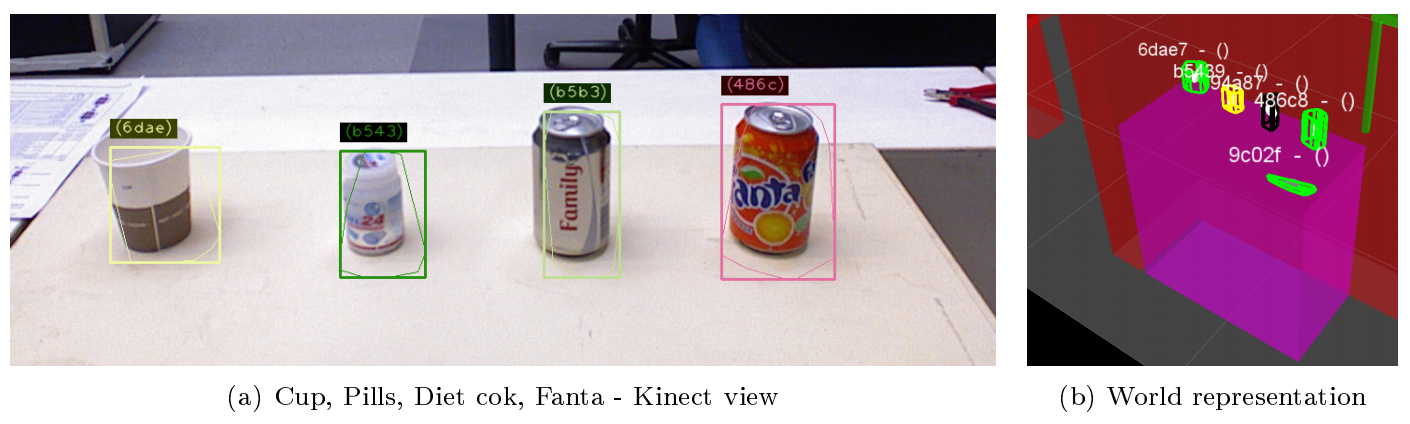
\includegraphics[width = \linewidth]{Figures/ed_perception}
	\label{fig:ed_perception}
\end{figure}
In order the classify or train unknown entities, the ed\_perception\footnote{\url{https://github.com/tue-robotics/ed_perception}} plugin exposes ROS Services. The following ROS Services are exposed:
\begin{enumerate}
	\item \textbf{AddTrainingInstance.srv} This service adds training data to an ed\_object\_model
	\item \textbf{Classify.srv} This service tries to classify an unknown entity in the scene. The following classifiers are used
	\begin{enumerate}
		\item Size matcher
		\item SIFT matcher
		\item Color matcher
		\item QR detector
		\item Face detector (face detection / template matching)
	\end{enumerate}
	\item \textbf{LearnPerson.srv} Service that learns the face of an entity in the scene
\end{enumerate}
For object recognition, the classify service is used. The classify services takes as an argument the id of the entity and returns the classification. This can either be a trained object or person or just the label “human”.
\begin{figure}[ht]
	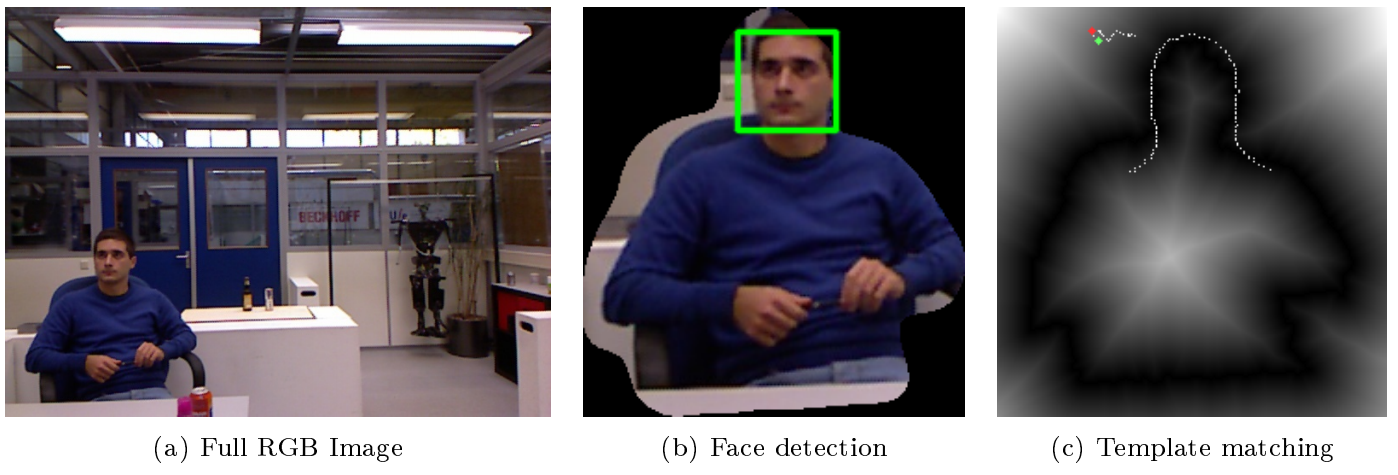
\includegraphics[width = \linewidth]{Figures/ed_perception_people}
	\label{fig:ed_perception_people}
\end{figure}
In order to create a new training set for specific objects, the ed\_perception package contains several tools for segmenting objects and annotation. 